%%%%%%%%%%%%%%%%%%%%%%%%%%%%%%%%%%%%%%%%%%%%%%%%%%%%%%%%%% 
\chapter{評価実験} \label{chap:exp}
%%%%%%%%%%%%%%%%%%%%%%%%%%%%%%%%%%%%%%%%%%%%%%%%%%%%%%%%%% 

本章では,ベンチマーク問題を使用した実験結果を通じて
提案する2種類のASP符号化の比較評価を行う.

ベンチマーク問題として,DNET\footnote{https://github.com/takemaru/dnet}
で公開されている配電網モデル3問と,
Graph Coloring and its Generalization\footnote{https://mat.tepper.cmu.edu/COLOR04/}
で公開されているグラフ彩色問題127問中,
辺の数が50000以下である非連結成分を含まない無向グラフ82問に対し,
ノードのうち1/5個をランダムに根として与えたものを用いた.
これらの計85問の問題のノードの数は11~1406,辺の数は16~49629,根の数は1~281である.

実験は,提案した2種類のASP符号化\code{srf1}(コード~\ref{code:srf1.lp}),
\code{srf2}(コード~\ref{code:srf2.lp})を用いて符号化した170問について,
それぞれ制限時間を1時間として{\clingo}で実行し,
解いた問題数,各問題の実行CPU時間と制約数を集計する.
なお,{\clingo}のバージョンは5.4.0,オプションとして\textsl{trendy}を使用した.
実験環境は,Mac mini,3.2 GHz Intel Core i7,64GBメモリである.

はじめに,各符号化の性能を比較するためにカクタスプロットによる比較結果を図~\ref{fig:cactus}に示す.
カクタスプロットは,縦軸が各問題を解くまでのCPU時間を表し,横軸が解けた問題数を表す.
グラフが右に寄るほど制限時間内に多くのベンチマーク問題を解くことが可能であることを意味するので,
符号化の性能が良いとされる.

%%%%%%%%%%%%%%%%%%%%%%%%%%%%%%
\begin{figure}[htbp]
 \centering
 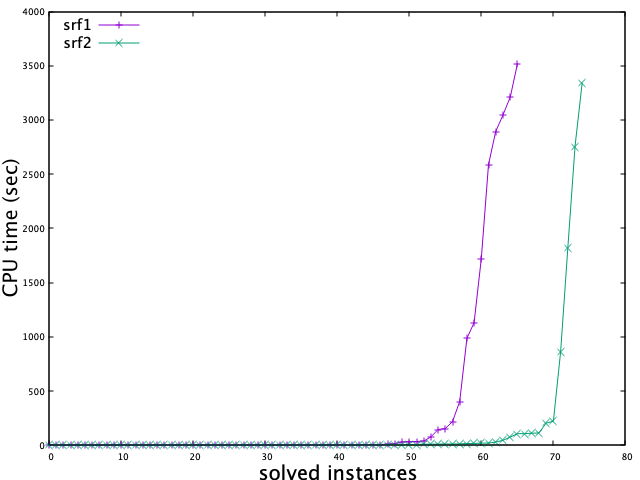
\includegraphics[scale=0.5]{fig/cactus.png}
 \caption{比較結果: カクタスプロット} 
 \label{fig:cactus}
\end{figure}
%%%%%%%%%%%%%%%%%%%%%%%%%%%%%%

結果では,\code{srf2}符号化は\code{srf1}符号化よりも解いた問題数が多いことを示した.
また,今回実験を行った多くの問題に対してASPによる全域森探索は実行CPU時間が小さいことを示した.

次に,実際に各符号化が解いた問題について,
問題の規模ごとに分類して比較したものを表\ref{table:kibo}に示す.
表中の太字は,解けた問題数を比較して多い方,または同数であることを表している.

%%%%%%%%%%%%%%%%%%%%%%%%%%%%%%
\begin{table}[htbp]
  \caption{比較結果: 解けた問題数(問)}
  \label{table:kibo}
  \centering
 \begin{tabular}[t]{c|c|c|c}
  \noalign{\hrule height 1pt}
  辺の数 & 問題数 & \code{srf1} & \code{srf2} \\
  \noalign{\hrule height 1pt}
%%%%%%%%
  1 ~ 1000 & 30 & \textbf{30} & \textbf{30} \\
  \hline
  1001 ~ 4000 & 20 & \textbf{20} & \textbf{20} \\
  \hline
  4001 ~ 7000 & 11 & 9 & \textbf{10} \\
  \hline
  7001 ~ 10000 & 8 & 4 & \textbf{6} \\
  \hline
  10001 ~ 20000 & 9 & 2 & \textbf{5} \\
  \hline
  20001 ~ 30000 & 2 & 1 & \textbf{2} \\
  \hline
  30001 ~ 40000 & 1 & 0 & 0 \\
  \hline
  40001 ~ 50000 & 4 & 0 & \textbf{2} \\
%%%%%%%% 合計
  \noalign{\hrule height 1pt}
  計 & 85 & 66 & \textbf{75} \\
  \noalign{\hrule height 1pt}
 \end{tabular}
\end{table}
%%%%%%%%%%%%%%%%%%%%%%%%%%%%%%

結果から,辺の数が少ない問題では符号化による解けた問題数の差は大きく見られないが,
辺の数が10,000を超える問題では,\code{srf2}の方が\code{srf1}よりも多くの問題を解いたことを示した.
また,\code{srf2}による符号化では,辺の数が40,000を超えるような大規模の問題に対して,
解を求めることに成功した.
これらの結果から,\ref{chap:prop}章で述べた\code{srf2}符号化の特長である,
根付き連結制約を符号化した際の制約数が少なく抑えられることが拡張性の高さに
有効であったといえる.

実際に\code{srf2}符号化の方が制約数が少ないことを確認するために,
辺の数が7000より大きい問題について,生成された制約数の比較結果を図\ref{fig:constraints}に示す.

\begin{figure}[htbp]
 \centering
 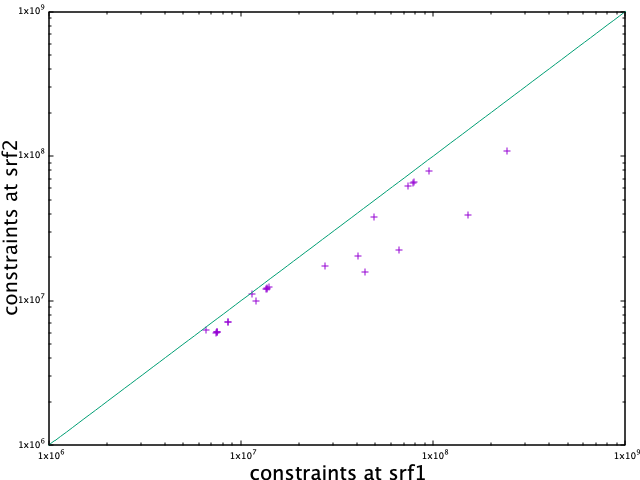
\includegraphics[scale=0.5]{fig/constraints.png}
 \caption{比較結果: 生成された制約数}
 \label{fig:constraints}
\end{figure}

図\ref{fig:constraints}は,横軸が\code{srf1}による制約数,縦軸が\code{srf2}による制約数を示す.
図中のラインは,2つの符号化の生成される制約数が同じになる境界を表している.
記号$+$は問題を表しており,その座標が各符号化の制約数となる.
記号が境界から下にあれば,その問題では\code{srf1}の方が制約数が少なくなることを意味する.
反対に,記号が境界から上にあれば,\code{srf2}の方が制約数が少なくなることを意味する.

結果を見ると,記号は全体的に境界よりも下にあるため,
確かに\code{srf2}による符号化は生成される制約の数が
少なく抑えられていることが確認できる.


%%% Local Variables:
%%% mode: japanese-latex
%%% TeX-master: "paper"
%%% End:
